\begin{frame}[fragile]{Tutorial: n-site states with MPS}

\begin{columns}

\begin{column}{5.5cm}

\begin{onlyenv}<1->
\begin{lstlisting}[language=JuliaLocal, style=julia, mathescape, basicstyle=\scriptsize\ttfamily]
$\psi$0 = MPS(i, "Zp")
nlayers = 6
function F($\theta$)
  $\psi\theta$=apply(U($\theta$,i;nlayers),$\psi$0)
  return -abs2(inner($\psi$',$\psi\theta$))
end

$\theta$0 = zeros(nlayers*n)
$\theta$ = minimize(F, $\partial$F, $\theta$0;
          nsteps=20, $\gamma$=0.1)
\end{lstlisting}
\end{onlyenv}

%% # 1 (product state)
%% # 2 (entangled state)
%% # (-0.556066, 0.895717)
%% # (-0.995230, 0.048939)

\begin{onlyenv}<2->
\begin{lstlisting}[language=JuliaLocal, style=julia, mathescape, basicstyle=\scriptsize\ttfamily]
maxlinkdim($\psi$0) == 1
maxlinkdim($\psi\theta$) == 2
F($\theta$0) # $\approx$ -0.556066
F($\theta$) # $\approx$ -0.995230
\end{lstlisting}
\end{onlyenv}

\end{column}

\begin{column}{4.5cm}

%% \begin{onlyenv}<1-1>
%% 
%% \begin{lstlisting}[style=julia, numbers=none, mathescape, basicstyle=\scriptsize\ttfamily]
%% # |0$\rangle$ = |Z+Z+…Z+$\rangle$
%% 
%% # Minimize over $\theta$:
%% # F($\theta$) = -|$\langle\psi$|U($\theta$)|0$\rangle$|$^2$
%% #        = -|$\langle\psi$|$\theta\rangle$|$\^2$
%% 
%% 
%% 
%% 
%%  \end{lstlisting}
%% 
%% \end{onlyenv}

\begin{onlyenv}<1->
\vspace*{0.0cm}
\begin{center}
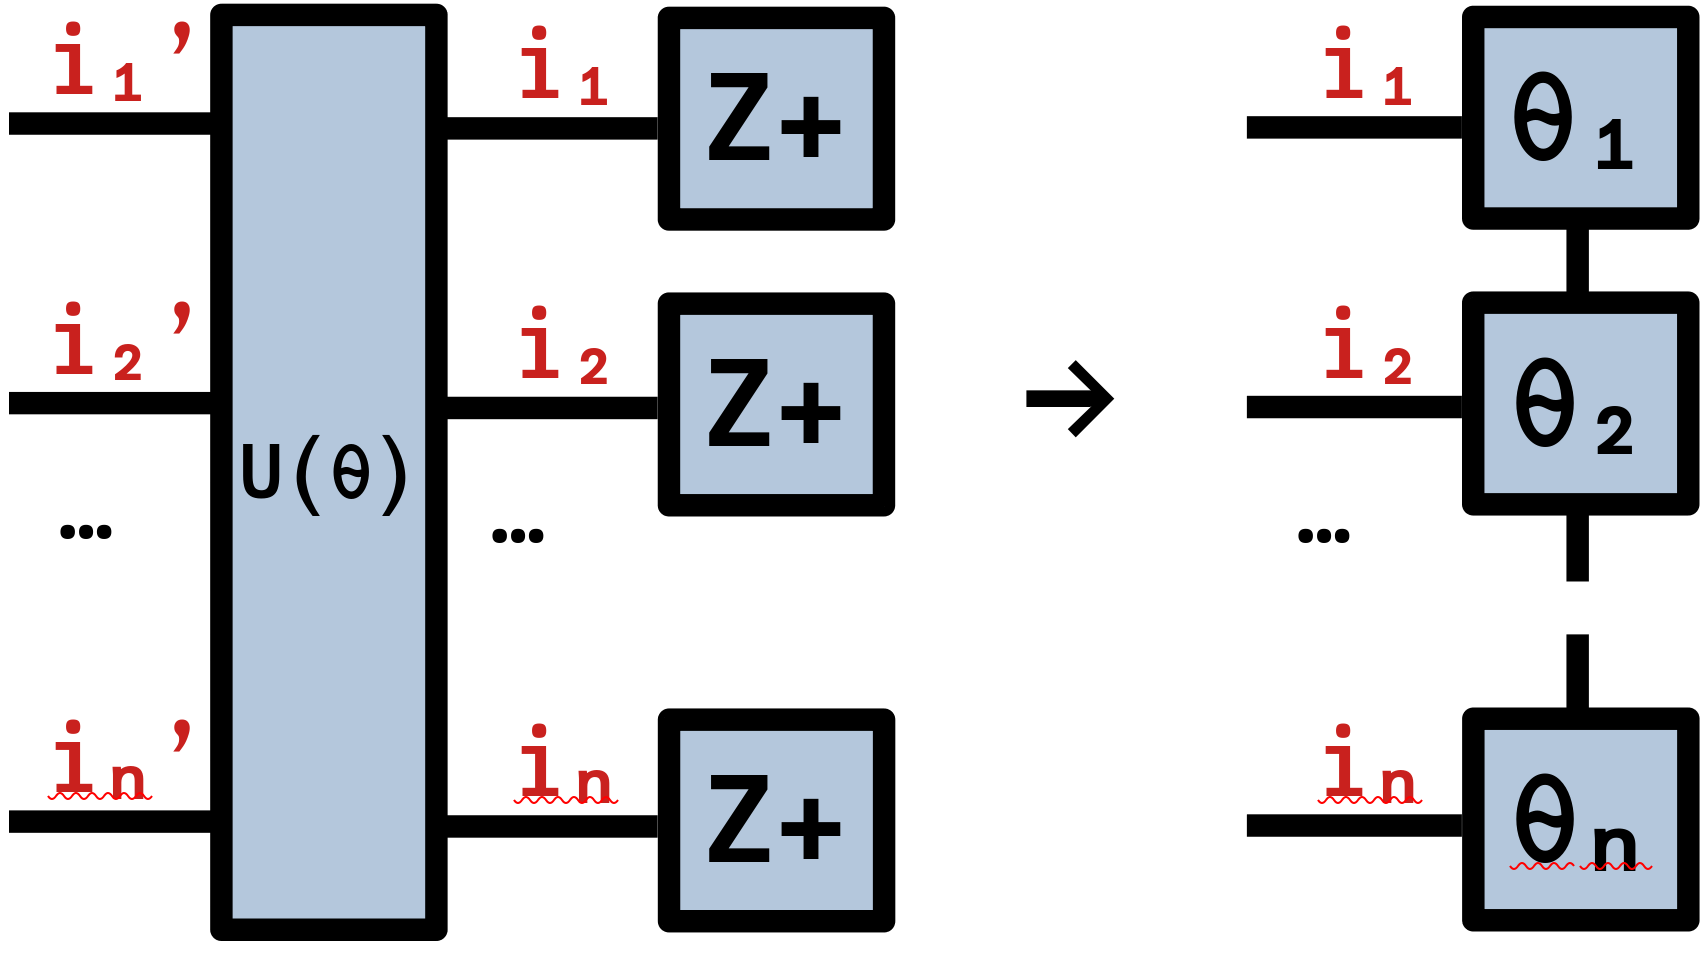
\includegraphics[width=\textwidth]{
  slides/assets/U_Zpn.png
} \\
~\\
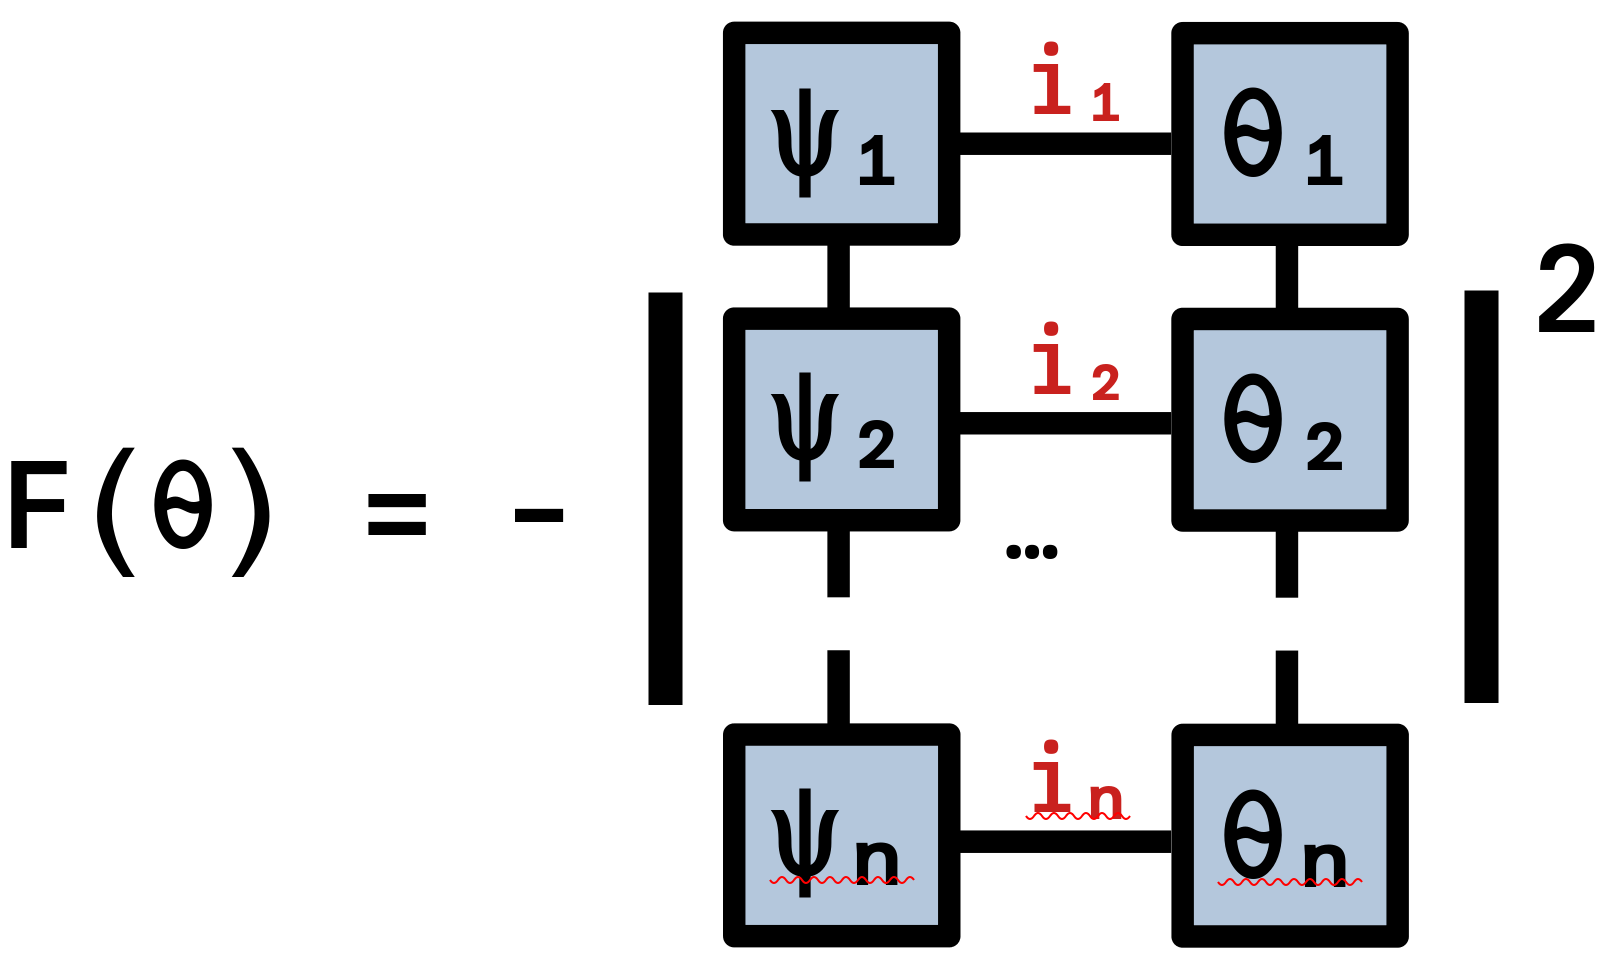
\includegraphics[width=\textwidth]{
  slides/assets/psin_thetan.png
} \\
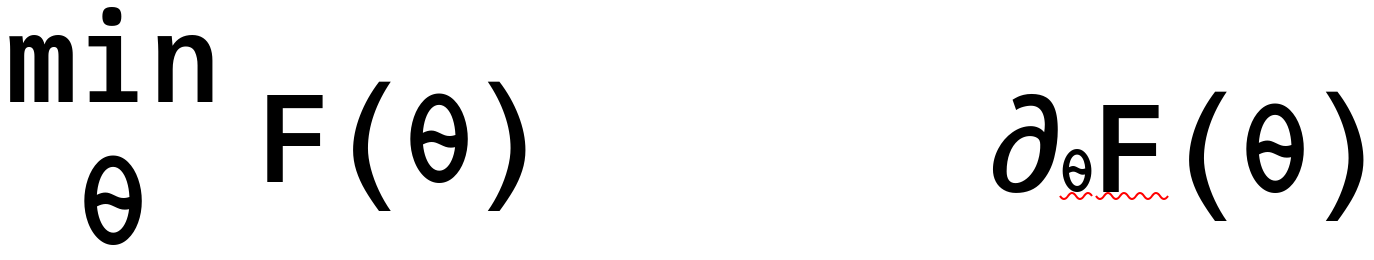
\includegraphics[width=\textwidth]{
  slides/assets/min_grad_F_theta.png
}
\end{center}
\vspace*{0.0cm}
\end{onlyenv}

%% \begin{onlyenv}<3->
%% \begin{lstlisting}[style=julia, numbers=none, mathescape, basicstyle=\scriptsize\ttfamily]
%% # 1 (product state)
%% # 2 (entangled state)
%% # (-0.556066, 0.895717)
%% # (-0.995230, 0.048939)
%% \end{lstlisting}
%% \end{onlyenv}

\end{column}

\end{columns}

\end{frame}
